Il modello a shell è un tentativo di mettere insieme un modello quantisticamente coerente di interazioni nucleari delle caratteristiche viste in precedenza. Le informazioni ottenute sul potenziale di interazione nucleone-nucleone vengono usate concretamente nel \textbf{modello shell}: si assumono i nucleoni all'interno di un potenziale efficace ridotto dagli altri nucleoni. Si avrà una definizione dei livelli energetici, spin e momenti magnetici. Questo è sostanzialmente un approccio simile alle strutture a shell degli atomi ma con significative differenze. Siamo in caso di potenziale a breve range, non esiste il potenziale coulombiano del nucleo: i nucleoni producono e subiscono il potenziale e le interazioni spin-spin e spin-orbita molto più rilevanti.
\subsection{Numeri magici}
%IMMAGINE magi
\begin{figure}[htp!]
  \centering
  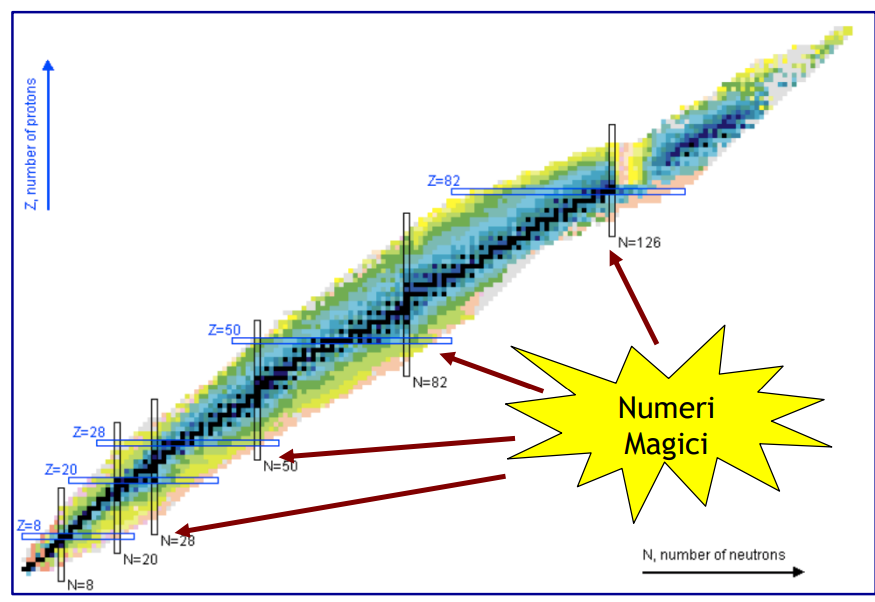
\includegraphics[scale=0.4]{Lezione7/magi.png} 
\end{figure}
Se uno va a vedere in dettaglio questa struttura nota che ci sono dei numeri particolari di $Z$ o di $N$ in cui c'è un'abbondanza di nuclei stabili. Dei massimi di energia di legame per nucleone che corrisponde a valori ben specifici di $N$ e di $Z$. La formula dell'energia di legame questo comportamento non riesce a spiegarlo. Questi numeri vengono detti \textbf{numeri magici}. Addirittura il nucleo più grosso stabile ($\ch{^{208}Pb}$) è detto \textbf{bi-magico} in quanto ha due numeri magici sia $Z=82$ che $N=126$. 
\subsection{Modello a shell atomico}
Nel modello dell'atomo a idrogeno, l'energia dipende dalla somma $n+l$:
\begin{equation*}
    E_n=\left(\frac{e^2}{4\pi\varepsilon_0\hbar c}\right)^2\frac{m_ec^2}{2(n+l)^2}=\alpha^2\frac{m_ec^2}{2(n+l)^2}
\end{equation*}
Stati degeneri che hanno diverso momento angolare. Questa degenerazione che è specifica per il caso $1/r$ è rimossa quando si considerano perturbazioni al puro potenziale $1/r$: presenza di altri elettroni che modificano il potenziale, oppure l'interazione spin-orbita. Un'altra osservazione è che l'energia di legame e dimensione atomica ($R$ decresce all'aumentare di $Z$) presentano transizioni brusche quando si passa al livello successivo.
%IMMAGINE dsds gg
\begin{figure}[htp!]
  \centering
  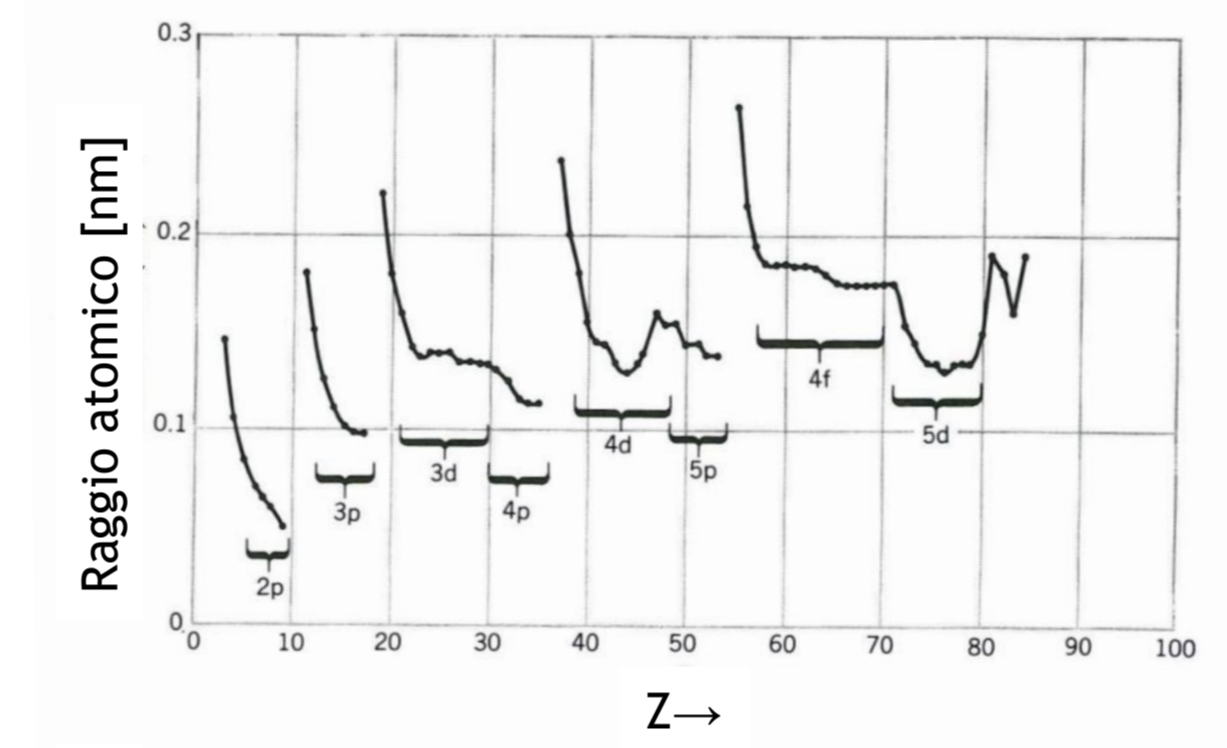
\includegraphics[scale=0.1]{Lezione7/kk.jpg}
  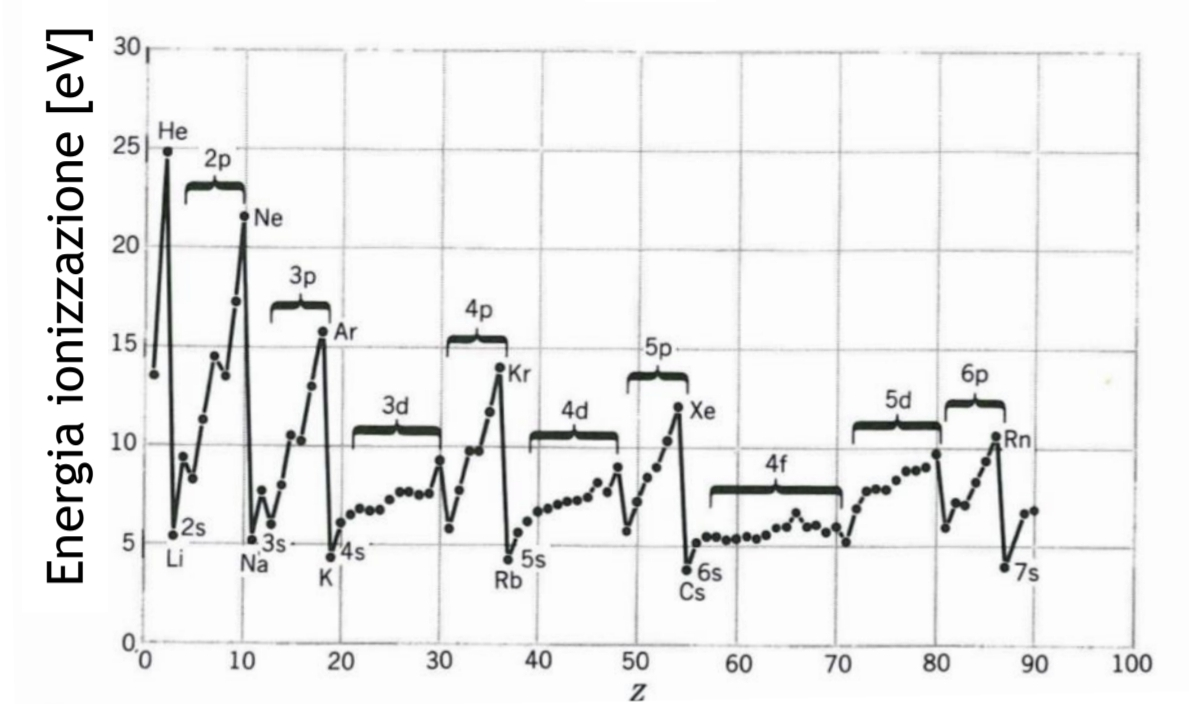
\includegraphics[scale=0.1]{Lezione7/zz.jpg} 
\end{figure}
\subsection{Potenziale nucleare}
Ritornando al nucleo visto che abbiamo interazioni a breve range possiamo dire che il potenziale varia in base alla densità di materia all'interno del nucleo:
\begin{equation*}
    V(r)=\frac{-V_0}{1+\text{exp}{[(r-R)/a]}}
\end{equation*}
Questa densità in teoria sappiamo circa come è fatta grazie agli esperimenti di Hofstdader dove si è andati a mappare l'interno dei nuclei. Dove all'interno è circa costante mentre appena si arriva al bordo decresce in maniera esponenziale (andandomi a sbrodolare il fatto che il nucleo finisce istantaneamente) e quindi abbiamo la soluzione a cappello. Quindi questo aspetto si descrive andando a prendere un potenziale che ribalta questa cosa:
dove $V_0$ è la profondità della buca (abbiamo detto circa $35\,MeV$), $R$ è l'estensione del nucleo e $a$ è la dimensione dello strato superficiale (che se vogliamo possiamo pensarlo come il range della mia interazione). Quindi per $r\to\infty$ questo potenziale tende a $0$. Il denominatore mi da questa decrescita del potenziale della densità quando esco dal nucleo.
%IMMAGINE pot nm
\begin{figure}[htp!]
  \centering
  
\includegraphics[scale=0.5]{Lezione7/pot.png}
  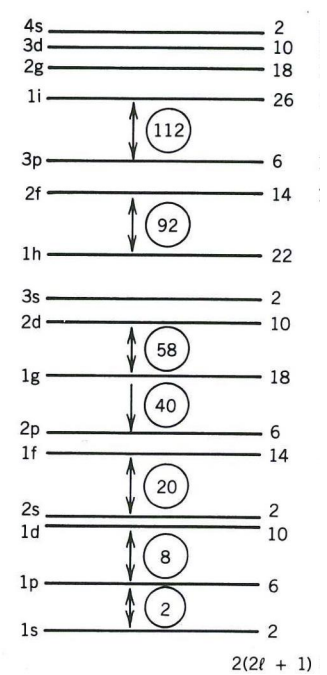
\includegraphics[scale=0.4]{Lezione7/nm.png} 
\end{figure}
Il $2(2l+1)$ numero di stati possibile ad ogni livello rappresenta il fatto che per il principio di esclusione di Pauli non posso avere nello stesso livello due fermioni che hanno gli stessi numeri quantici. I numeri quantici che posso differire per fermini nello stesso livello sono: la componente $z$ del momento angolare e la componente $z$ dello spin. Quindi sostanzialmente il $2l+1$ mi dice quanti possibili valori di $L_z$ del momento angolare, moltiplicato per $2$ i due possibili valori dello spin. I numeri in grosso cerchiati sono le particelle che ho raggruppato fino a quel livello.
Si può risolvere l'equazione di Schr\"odinger con questo potenziale e quello che otteniamo sono dei livelli energetici nettamente quindi non è presente la degenerazione presente nel modello orbitale atomico.
Compaiono salti a certi valori di nucleoni: \textbf{numeri magici}: non sono però corretti. Infatti $40,\, 58,\, 92,\, 112$ non sono i numeri magici che compaiono nella carta dei nuclidi e mancano altri valor: $28,\,50,\,82,\,126$.

Quindi dopo il potenziale radiale un altro ingrediente importante è l'interazione spin-orbita.
\subsection{Interazione spin-orbita}
Piccola premessa: ora si tratterà un'analogia con le interazione elettromagnetiche per seguire meglio il filo del discorso ma ovviamente l'intensità è diversa. Il modello intuitivo è prendere un nucleone in uno stato con momento orbitale $\mathbf{L}$ che vede un momento magnetico (perchè è praticamente un oggetto che orbita). Quindi ad un momento orbitale posso associare un momento magnetico (che sarà proporzionale a questo momento orbitale):
\begin{equation*}
    \bm{\mu}_L\propto \mu_N\mathbf{L}
\end{equation*}
%IMMAGINE orb
\begin{figure}[htp!]
  \centering
  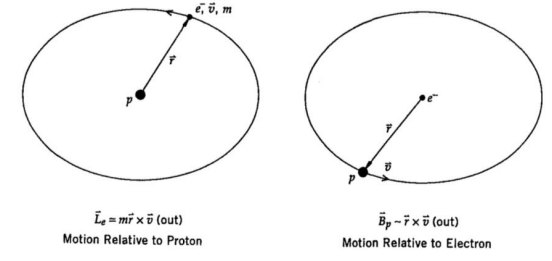
\includegraphics[scale=0.9]{Lezione7/orb.png} 
\end{figure}
Questo momento magnetico interagirà con lo spin del nucleone a dare un termine energetico:
\begin{equation*}
    U\propto-\mathbf{L}\cdot\mathbf{S}
\end{equation*}
Quindi ogni livello si divide in due sottolivelli con un momento angolare totale (eccetto $l=0$) questo perchè lo spin può essere parallelo o antiparallelo.
\begin{equation*}
    J=l+\frac{1}{2}\qquad J=l-\frac{1}{2}
\end{equation*}
\subsubsection{Interazione spin-orbita}
Un momento magnetico, immerso in un campo magnetico acquista un'energia potenziale:
\begin{equation*}
    U=-\bm{\mu}\cdot\mathbf{B}
\end{equation*}
A sua volta genera un campo magnetico:
\begin{equation*}
    \mathbf{B}=\frac{\mu_0}{4\pi}\left[\frac{3(\bm{\mu}\cdot\hat{\mathbf{r}})\hat{\mathbf{r}}-\bm{\mu}}{r^3}\right]
\end{equation*}
L'interazione tra due dipoli è dunque della forma:
\begin{equation*}
    U=-\frac{\mu_0}{4\pi}\left[\frac{3(\bm{\mu}_1\cdot\hat{\mathbf{r}})(\bm{\mu}_2\cdot\hat{\mathbf{r}})-\bm{\mu}_1\cdot\bm{\mu}_2}{r^3}\right]
\end{equation*}
Come ordine di grandezza dell'interazione avremo qualcosa dell'ordine del $\sim 3.4\,keV$. Per elettroni atomici: $\sim 6\times10^{-3}\,eV$.
\subsection{Interazione spin-orbita}
Da un punto di vista sperimentale risulta energeticamente favorebole l'allineamento di spin e momento angolare orbitale. Abbiamo detto essere proporzionale a:
\begin{equation*}
    \mathbf{L}\cdot\mathbf{S}=\frac{1}{2}\left[\mathbf{J}^2-\mathbf{L}^2-\mathbf{S}^2\right]=\frac{1}{2}[J(J+1)-l(l+1)-s(s+1)]
\end{equation*}
La separazione tra i livelli:
\begin{align*}
    \Delta\left(\mathbf{L}\cdot\mathbf{S}\right)=J_{l+s}(J_{l+s}+1)-J_{l-s}(J_{l-s}+1)= \\
    =\left(l+\frac{1}{2}\right)\left(l+\frac{2}{3}\right)-\left(l-\frac{1}{2}\right)\left(l+\frac{1}{2}\right)=2\left(l+\frac{1}{2}\right)
\end{align*}
$l$ ed $s$ singolarmente rimangono costanti e non cambiano quindi si cancellano. Tutta la differenza si concentra nei valori di $J$. Quello che vediamo è che questa differenza aumenta all'aumentare di $l$. Più grande è $l$ più i due livelli energetici si stanno separando. Ma questo ce lo aspettavamo. La variazione dei numeri magici viene giustificata proprio che all'aumentare di $l$ la separazione diventa importante e mi va a scombinare l'ordine dei livelli energetici. 

Abbiamo visto anche \textbf{l'interazione spin-spin} che come abbiamo visto nell'interazione nucleone-nucleone ci deve essere anche un termine di accoppiamento spin-spin di due nucleoni: \textbf{energia di pairing}. Questo favorisce l'anti-allineamento dei due spin, risultato in uno stato con spin totale $0$. Quindi tutti i nuclei pari-pari hanno stato fondamentale con $J=0$ questo perchè se io prendo le particelle in un certo livello energetico e queste le posso mettere a coppie due-due, questa energia di pairing mi porta ad avere i due spin opposti, siccome ho un certo valore fissato di $J$ se ho due spin opposti anche il $J$ è oppposto e quindi i due momenti di cancellano e il momento totale si annulla. Il risultato del modello a shell e questa divisione dei momenti:
%IMMAGINE ff
\begin{figure}[htp!]
  \centering
  
\includegraphics[scale=0.5]{Lezione7/ff.png} 
\end{figure}
\subsection{La formula di Bethe-Weizs\"acker}
Possiamo adesso vedere come questa teoria giustifica gli ultimi due termini della formula di Bethe-Weizs\"acker:
\begin{equation*}
    \text{B.E.}(A,Z)=-a_{1}A+a_{2}A^{\frac{2}{3}}+a_{3}{\frac {Z^2}{A^{\frac{1}{3}}}}+a_{4}{\frac {(N-Z)^{2}}{A}}\pm a_5 A^{-\frac{3}{4}}
\end{equation*}
Gli ultimi due termini non hanno un analogo classico e vengono introdotti fenomenologicamente. Il quarto termine tiene conto del fatto che i nuclei sono più stabili quando c'è \textbf{simmetria fra protoni e neutroni: }$\mathbf{N}\sim\mathbf{Z}$. Descrive la \textbf{valle di stabilità}.

Per il \textbf{Principio di esclusione di Pauli}: due particelle con $s=1/2$ non possono avere gli stessi numeri quantici ad esempio:
%IMMAGINE es
\begin{figure}[htp!]
  \centering
  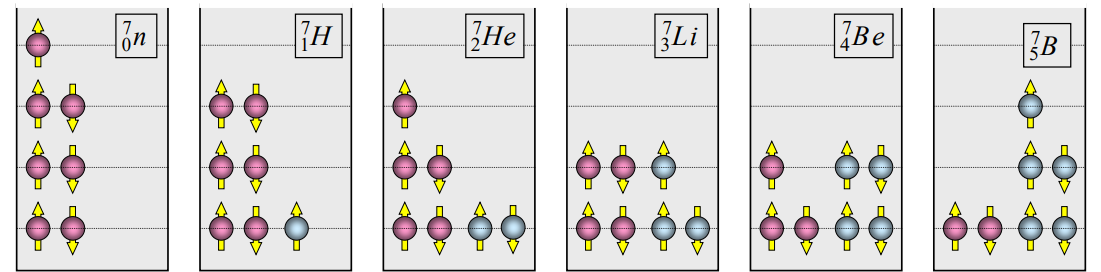
\includegraphics[scale=0.5]{Lezione7/es.png} 
\end{figure}
Se io ho un certo livello ben specifico posso metterci massimo due particelle perchè posso separare e distinguere due nucleoni identici solamente attraverso l'orientamento dello spin. Ad esempio se cercassi di fare un nucleo con $7$ neutroni sarei obbligato a mettere i primi due al primo livello ma i successivi in livelli energetici sempre maggiori. Successivamente se converto un neutrone in un protone, il protone può stare nel livello energetico più basso in quanto è diverso. Questa configurazione avrebbe un'energia molto più bassa quindi energeticamente favorevole. Questa cosa mi continua fino a quando raggiungo una condizione di minima energia. Queste considerazioni ci giustificano il fatto che attraverso discorsi energetici andiamo a preferire nulcei con un numero di protoni e neutroni simile spiegando il quarto termine della formula di Bethe-Weizs\"acker. Dal punto di vista del principio di esclusione di Pauli gli stati intermedi in cui ho un minimo di energia sono equivalenti anche se in realtà per i protoni abbiamo la repulsione coulombiana e di conseguenza la configurazione con $Z$ più alto sarà leggermente più sfavorito. 

Il fatto che la valle di stabilità inizia a piegarsi è dovuto all'effetto coulombiano che inizia a predominare su questo effetto dovuto al principio di esclusione di Pauli.

Il quinto termine tiene conto del \textbf{pairing} degli spin. Infatti è \textbf{nullo} per $A$ dispari, \textbf{negativo} quando $N$ e $Z$ sono pari (nuclei pari-pari) e \textbf{positivo} quando $N$ e $Z$ sono dispari (nuclei dispari-dispari).
%IMMAGINE tt
\begin{figure}[htp!]
  \centering
  
\includegraphics[scale=0.5]{Lezione7/tt.png} 
\end{figure}
Banalmente per quanto riguarda il deuterio abbiamo visto che come non possiamo mettere due protoni insieme (per ovvi motivi) non possiamo fare la stessa cosa con i neutroni.
\subsubsection{Momento di dipolo mangetico}
Nei nuclei con A-dispari, spin e momento magnetico sono determinati dal nucleone "spaiato". Ripetendo il discorso fatto per il deutone:
\begin{equation*}
    \bm{\mu}=g\mu_N\mathbf{J}=g_l\mu_N\mathbf{L}+g_s\mu_N\mathbf{S}
\end{equation*}
Per determinare il coefficiente giromagnetico, si può moltiplicare per $\mathbf{J}/\hbar$:
\begin{equation*}
    g\mathbf{J}^2=g_l\left(\mathbf{L}\cdot\mathbf{J}\right)+g_s\left(\mathbf{S}\cdot\mathbf{J}\right)
\end{equation*}
\begin{equation*}
    g=\frac{1}{j(j+1)}\left[g_l\left(\mathbf{L}^2+\mathbf{L}\cdot\mathbf{S}\right)+g_s\left(\mathbf{S}^2+\mathbf{S}\cdot\mathbf{L}\right)\right]=\ldots
\end{equation*}
Da qui posso ottenere il valore di $g$ per $j=l\pm1/2$.
\subsection{Eccitazioni collettive}
Per nuclei grandi il modello a shell ricude il suo valore predittivo. Eccitazioni dei nuclei più esterni possono trasferirsi agli orbitali meno legati ed eccitare movimenti degli altri nucleoni. Questi sono i moti collettivi dei nucleoni in cui il nucleo si deforma. Quindi moti vibrazionali o moti rotazionali.
